\begin{frame}[fragile]{Visualização de RSQ(2, 6)}

    \begin{figure}
        \centering

        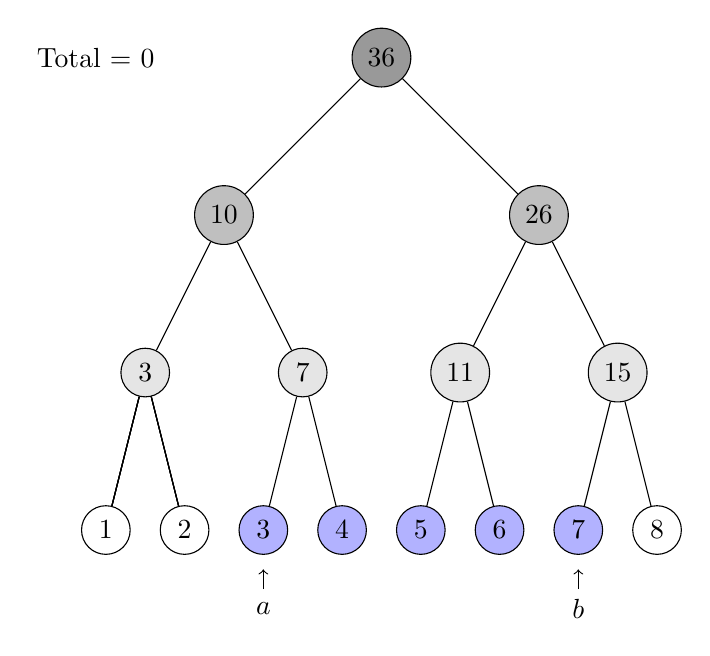
\begin{tikzpicture}
            \node[anchor=west] at (0, 6) { Total = $0$ };

            \node at (3, -1) { $a$ };
            \node at (7, -1) { $b$ };

            \draw[->] (3, -0.75) -- (3, -0.5);
            \draw[->] (7, -0.75) -- (7, -0.5);

            \node[draw,circle] (A1) at (1, 0) { 1 };
            \node[draw,circle] (A2) at (2, 0) { 2 };
            \node[draw,circle,fill=blue!30] (A3) at (3, 0) { 3 };
            \node[draw,circle,fill=blue!30] (A4) at (4, 0) { 4 };
            \node[draw,circle,fill=blue!30] (A5) at (5, 0) { 5 };
            \node[draw,circle,fill=blue!30] (A6) at (6, 0) { 6 };
            \node[draw,circle,fill=blue!30] (A7) at (7, 0) { 7 };
            \node[draw,circle] (A8) at (8, 0) { 8 };

            \node[draw,circle,fill=gray!20] (B1) at (1.5, 2) { 3 };
            \node[draw,circle,fill=gray!20] (B2) at (3.5, 2) { 7 };
            \node[draw,circle,fill=gray!20] (B3) at (5.5, 2) { 11 };
            \node[draw,circle,fill=gray!20] (B4) at (7.5, 2) { 15 };

            \node[draw,circle,fill=gray!50] (C1) at (2.5, 4) { 10 };
            \node[draw,circle,fill=gray!50] (C2) at (6.5, 4) { 26 };

            \node[draw,circle,fill=gray!80] (D1) at (4.5, 6) { 36 };

            \draw (A1) -- (B1);
            \draw (A2) -- (B1);
            \draw (A3) -- (B2);
            \draw (A4) -- (B2);
            \draw (A5) -- (B3);
            \draw (A6) -- (B3);
            \draw (A7) -- (B4);
            \draw (A8) -- (B4);
            \draw (A1) -- (B1);
            \draw (A2) -- (B1);
            \draw (A1) -- (B1);
            \draw (A2) -- (B1);
            \draw (A1) -- (B1);
            \draw (A2) -- (B1);
            \draw (B1) -- (C1);
            \draw (B2) -- (C1);
            \draw (B3) -- (C2);
            \draw (B4) -- (C2);
            \draw (C1) -- (D1);
            \draw (C2) -- (D1);
        \end{tikzpicture}
    \end{figure}

\end{frame}

\begin{frame}[fragile]{Visualização de RSQ(2, 6)}

    \begin{figure}
        \centering

        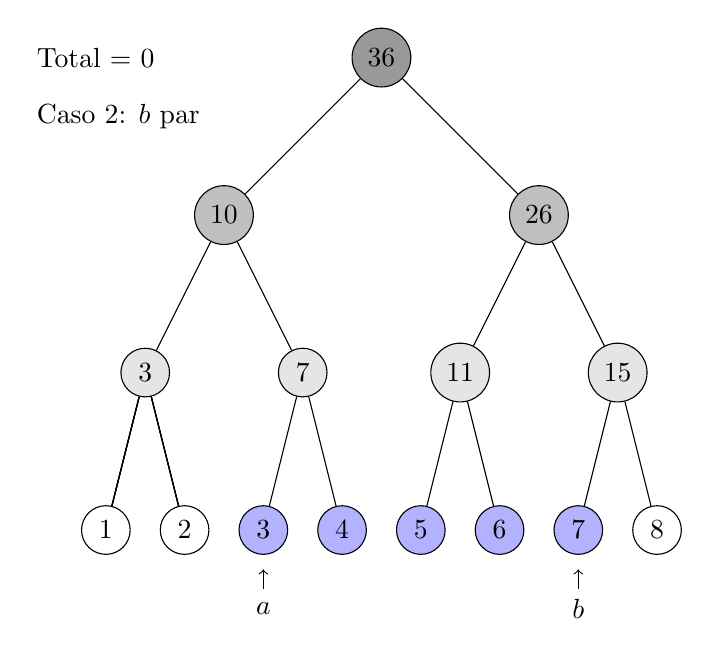
\begin{tikzpicture}
            \node[anchor=west] at (0, 6) { Total = $0$ };
            \node[anchor=west] at (0, 5.25) { Caso 2: $b$ par };

            \node at (3, -1) { $a$ };
            \node at (7, -1) { $b$ };

            \draw[->] (3, -0.75) -- (3, -0.5);
            \draw[->] (7, -0.75) -- (7, -0.5);

            \node[draw,circle] (A1) at (1, 0) { 1 };
            \node[draw,circle] (A2) at (2, 0) { 2 };
            \node[draw,circle,fill=blue!30] (A3) at (3, 0) { 3 };
            \node[draw,circle,fill=blue!30] (A4) at (4, 0) { 4 };
            \node[draw,circle,fill=blue!30] (A5) at (5, 0) { 5 };
            \node[draw,circle,fill=blue!30] (A6) at (6, 0) { 6 };
            \node[draw,circle,fill=blue!30] (A7) at (7, 0) { 7 };
            \node[draw,circle] (A8) at (8, 0) { 8 };

            \node[draw,circle,fill=gray!20] (B1) at (1.5, 2) { 3 };
            \node[draw,circle,fill=gray!20] (B2) at (3.5, 2) { 7 };
            \node[draw,circle,fill=gray!20] (B3) at (5.5, 2) { 11 };
            \node[draw,circle,fill=gray!20] (B4) at (7.5, 2) { 15 };

            \node[draw,circle,fill=gray!50] (C1) at (2.5, 4) { 10 };
            \node[draw,circle,fill=gray!50] (C2) at (6.5, 4) { 26 };

            \node[draw,circle,fill=gray!80] (D1) at (4.5, 6) { 36 };

            \draw (A1) -- (B1);
            \draw (A2) -- (B1);
            \draw (A3) -- (B2);
            \draw (A4) -- (B2);
            \draw (A5) -- (B3);
            \draw (A6) -- (B3);
            \draw (A7) -- (B4);
            \draw (A8) -- (B4);
            \draw (A1) -- (B1);
            \draw (A2) -- (B1);
            \draw (A1) -- (B1);
            \draw (A2) -- (B1);
            \draw (A1) -- (B1);
            \draw (A2) -- (B1);
            \draw (B1) -- (C1);
            \draw (B2) -- (C1);
            \draw (B3) -- (C2);
            \draw (B4) -- (C2);
            \draw (C1) -- (D1);
            \draw (C2) -- (D1);
        \end{tikzpicture}
    \end{figure}

\end{frame}

\begin{frame}[fragile]{Visualização de RSQ(2, 6)}

    \begin{figure}
        \centering

        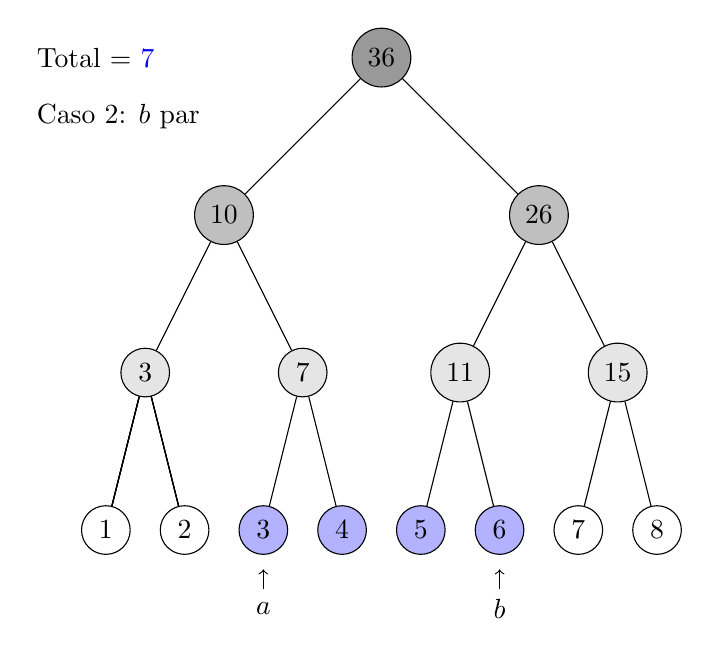
\begin{tikzpicture}
            \node[anchor=west] at (0, 6) { Total = \textcolor{blue}{$7$} };
            \node[anchor=west] at (0, 5.25) { Caso 2: $b$ par };

            \node at (3, -1) { $a$ };
            \node at (6, -1) { $b$ };

            \draw[->] (3, -0.75) -- (3, -0.5);
            \draw[->] (6, -0.75) -- (6, -0.5);

            \node[draw,circle] (A1) at (1, 0) { 1 };
            \node[draw,circle] (A2) at (2, 0) { 2 };
            \node[draw,circle,fill=blue!30] (A3) at (3, 0) { 3 };
            \node[draw,circle,fill=blue!30] (A4) at (4, 0) { 4 };
            \node[draw,circle,fill=blue!30] (A5) at (5, 0) { 5 };
            \node[draw,circle,fill=blue!30] (A6) at (6, 0) { 6 };
            \node[draw,circle] (A7) at (7, 0) { 7 };
            \node[draw,circle] (A8) at (8, 0) { 8 };

            \node[draw,circle,fill=gray!20] (B1) at (1.5, 2) { 3 };
            \node[draw,circle,fill=gray!20] (B2) at (3.5, 2) { 7 };
            \node[draw,circle,fill=gray!20] (B3) at (5.5, 2) { 11 };
            \node[draw,circle,fill=gray!20] (B4) at (7.5, 2) { 15 };

            \node[draw,circle,fill=gray!50] (C1) at (2.5, 4) { 10 };
            \node[draw,circle,fill=gray!50] (C2) at (6.5, 4) { 26 };

            \node[draw,circle,fill=gray!80] (D1) at (4.5, 6) { 36 };

            \draw (A1) -- (B1);
            \draw (A2) -- (B1);
            \draw (A3) -- (B2);
            \draw (A4) -- (B2);
            \draw (A5) -- (B3);
            \draw (A6) -- (B3);
            \draw (A7) -- (B4);
            \draw (A8) -- (B4);
            \draw (A1) -- (B1);
            \draw (A2) -- (B1);
            \draw (A1) -- (B1);
            \draw (A2) -- (B1);
            \draw (A1) -- (B1);
            \draw (A2) -- (B1);
            \draw (B1) -- (C1);
            \draw (B2) -- (C1);
            \draw (B3) -- (C2);
            \draw (B4) -- (C2);
            \draw (C1) -- (D1);
            \draw (C2) -- (D1);
        \end{tikzpicture}
    \end{figure}

\end{frame}

\begin{frame}[fragile]{Visualização de RSQ(2, 6)}

    \begin{figure}
        \centering

        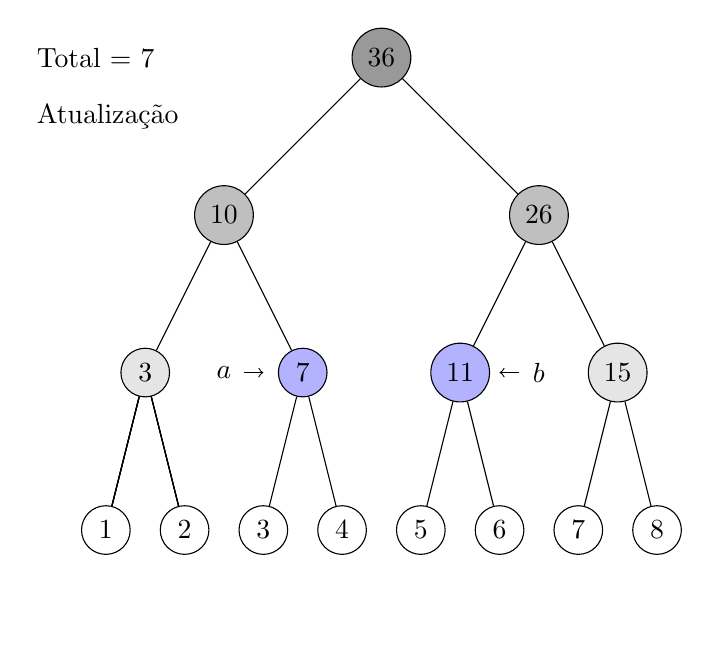
\begin{tikzpicture}
            \node[anchor=west] at (0, 6) { Total = \textcolor{black}{$7$} };
            \node[anchor=west] at (0, 5.25) { Atualização };

            \node at (2.5, 2) { $a$ };
            \node at (6.5, 2) { $b$ };
            \node[opacity=0] at (3, -1) { $a$ };
            \node[opacity=0] at (6, -1) { $b$ };

            \draw[->] (2.75, 2) -- (3, 2);
            \draw[->] (6.25, 2) -- (6, 2);

            \node[draw,circle] (A1) at (1, 0) { 1 };
            \node[draw,circle] (A2) at (2, 0) { 2 };
            \node[draw,circle] (A3) at (3, 0) { 3 };
            \node[draw,circle] (A4) at (4, 0) { 4 };
            \node[draw,circle] (A5) at (5, 0) { 5 };
            \node[draw,circle] (A6) at (6, 0) { 6 };
            \node[draw,circle] (A7) at (7, 0) { 7 };
            \node[draw,circle] (A8) at (8, 0) { 8 };

            \node[draw,circle,fill=gray!20] (B1) at (1.5, 2) { 3 };
            \node[draw,circle,fill=blue!30] (B2) at (3.5, 2) { 7 };
            \node[draw,circle,fill=blue!30] (B3) at (5.5, 2) { 11 };
            \node[draw,circle,fill=gray!20] (B4) at (7.5, 2) { 15 };

            \node[draw,circle,fill=gray!50] (C1) at (2.5, 4) { 10 };
            \node[draw,circle,fill=gray!50] (C2) at (6.5, 4) { 26 };

            \node[draw,circle,fill=gray!80] (D1) at (4.5, 6) { 36 };

            \draw (A1) -- (B1);
            \draw (A2) -- (B1);
            \draw (A3) -- (B2);
            \draw (A4) -- (B2);
            \draw (A5) -- (B3);
            \draw (A6) -- (B3);
            \draw (A7) -- (B4);
            \draw (A8) -- (B4);
            \draw (A1) -- (B1);
            \draw (A2) -- (B1);
            \draw (A1) -- (B1);
            \draw (A2) -- (B1);
            \draw (A1) -- (B1);
            \draw (A2) -- (B1);
            \draw (B1) -- (C1);
            \draw (B2) -- (C1);
            \draw (B3) -- (C2);
            \draw (B4) -- (C2);
            \draw (C1) -- (D1);
            \draw (C2) -- (D1);
        \end{tikzpicture}
    \end{figure}

\end{frame}

\begin{frame}[fragile]{Visualização de RSQ(2, 6)}

    \begin{figure}
        \centering

        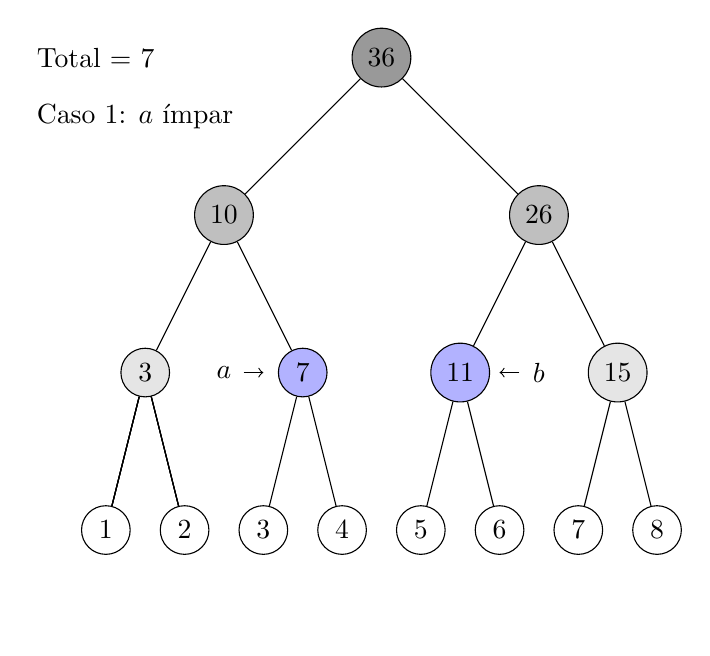
\begin{tikzpicture}
            \node[anchor=west] at (0, 6) { Total = \textcolor{black}{$7$} };
            \node[anchor=west] at (0, 5.25) { Caso 1: $a$ ímpar };

            \node at (2.5, 2) { $a$ };
            \node at (6.5, 2) { $b$ };
            \node[opacity=0] at (3, -1) { $a$ };
            \node[opacity=0] at (6, -1) { $b$ };

            \draw[->] (2.75, 2) -- (3, 2);
            \draw[->] (6.25, 2) -- (6, 2);

            \node[draw,circle] (A1) at (1, 0) { 1 };
            \node[draw,circle] (A2) at (2, 0) { 2 };
            \node[draw,circle] (A3) at (3, 0) { 3 };
            \node[draw,circle] (A4) at (4, 0) { 4 };
            \node[draw,circle] (A5) at (5, 0) { 5 };
            \node[draw,circle] (A6) at (6, 0) { 6 };
            \node[draw,circle] (A7) at (7, 0) { 7 };
            \node[draw,circle] (A8) at (8, 0) { 8 };

            \node[draw,circle,fill=gray!20] (B1) at (1.5, 2) { 3 };
            \node[draw,circle,fill=blue!30] (B2) at (3.5, 2) { 7 };
            \node[draw,circle,fill=blue!30] (B3) at (5.5, 2) { 11 };
            \node[draw,circle,fill=gray!20] (B4) at (7.5, 2) { 15 };

            \node[draw,circle,fill=gray!50] (C1) at (2.5, 4) { 10 };
            \node[draw,circle,fill=gray!50] (C2) at (6.5, 4) { 26 };

            \node[draw,circle,fill=gray!80] (D1) at (4.5, 6) { 36 };

            \draw (A1) -- (B1);
            \draw (A2) -- (B1);
            \draw (A3) -- (B2);
            \draw (A4) -- (B2);
            \draw (A5) -- (B3);
            \draw (A6) -- (B3);
            \draw (A7) -- (B4);
            \draw (A8) -- (B4);
            \draw (A1) -- (B1);
            \draw (A2) -- (B1);
            \draw (A1) -- (B1);
            \draw (A2) -- (B1);
            \draw (A1) -- (B1);
            \draw (A2) -- (B1);
            \draw (B1) -- (C1);
            \draw (B2) -- (C1);
            \draw (B3) -- (C2);
            \draw (B4) -- (C2);
            \draw (C1) -- (D1);
            \draw (C2) -- (D1);
        \end{tikzpicture}
    \end{figure}

\end{frame}

\begin{frame}[fragile]{Visualização de RSQ(2, 6)}

    \begin{figure}
        \centering

        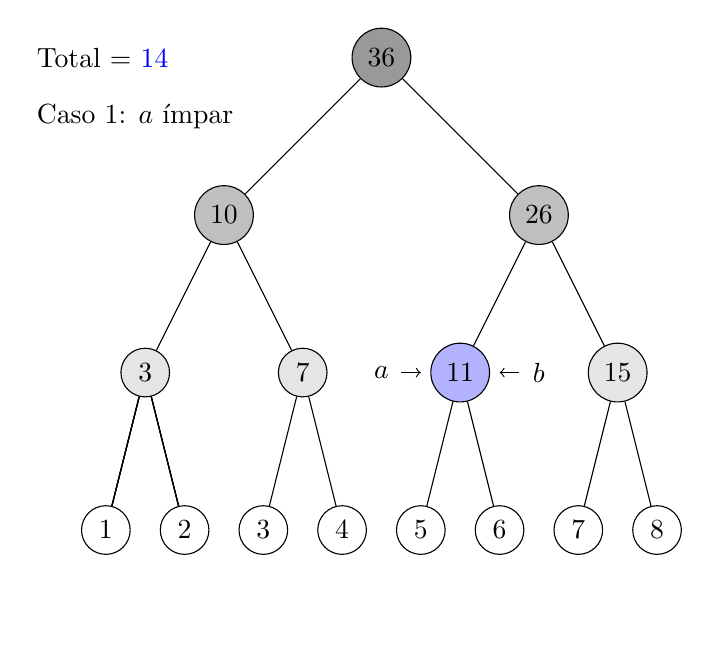
\begin{tikzpicture}
            \node[anchor=west] at (0, 6) { Total = \textcolor{blue}{$14$} };
            \node[anchor=west] at (0, 5.25) { Caso 1: $a$ ímpar };

            \node at (4.5, 2) { $a$ };
            \node at (6.5, 2) { $b$ };
            \node[opacity=0] at (3, -1) { $a$ };
            \node[opacity=0] at (6, -1) { $b$ };

            \draw[->] (4.75, 2) -- (5, 2);
            \draw[->] (6.25, 2) -- (6, 2);

            \node[draw,circle] (A1) at (1, 0) { 1 };
            \node[draw,circle] (A2) at (2, 0) { 2 };
            \node[draw,circle] (A3) at (3, 0) { 3 };
            \node[draw,circle] (A4) at (4, 0) { 4 };
            \node[draw,circle] (A5) at (5, 0) { 5 };
            \node[draw,circle] (A6) at (6, 0) { 6 };
            \node[draw,circle] (A7) at (7, 0) { 7 };
            \node[draw,circle] (A8) at (8, 0) { 8 };

            \node[draw,circle,fill=gray!20] (B1) at (1.5, 2) { 3 };
            \node[draw,circle,fill=gray!20] (B2) at (3.5, 2) { 7 };
            \node[draw,circle,fill=blue!30] (B3) at (5.5, 2) { 11 };
            \node[draw,circle,fill=gray!20] (B4) at (7.5, 2) { 15 };

            \node[draw,circle,fill=gray!50] (C1) at (2.5, 4) { 10 };
            \node[draw,circle,fill=gray!50] (C2) at (6.5, 4) { 26 };

            \node[draw,circle,fill=gray!80] (D1) at (4.5, 6) { 36 };

            \draw (A1) -- (B1);
            \draw (A2) -- (B1);
            \draw (A3) -- (B2);
            \draw (A4) -- (B2);
            \draw (A5) -- (B3);
            \draw (A6) -- (B3);
            \draw (A7) -- (B4);
            \draw (A8) -- (B4);
            \draw (A1) -- (B1);
            \draw (A2) -- (B1);
            \draw (A1) -- (B1);
            \draw (A2) -- (B1);
            \draw (A1) -- (B1);
            \draw (A2) -- (B1);
            \draw (B1) -- (C1);
            \draw (B2) -- (C1);
            \draw (B3) -- (C2);
            \draw (B4) -- (C2);
            \draw (C1) -- (D1);
            \draw (C2) -- (D1);
        \end{tikzpicture}
    \end{figure}

\end{frame}

\begin{frame}[fragile]{Visualização de RSQ(2, 6)}

    \begin{figure}
        \centering

        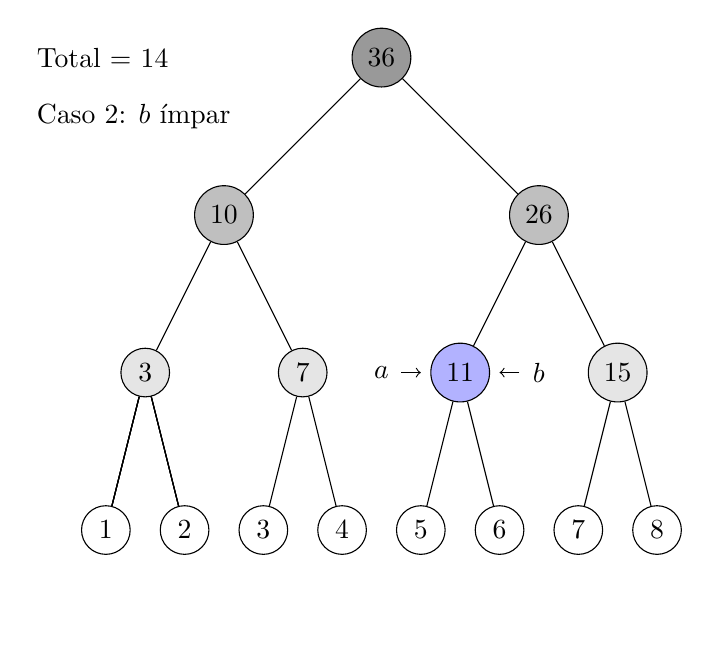
\begin{tikzpicture}
            \node[anchor=west] at (0, 6) { Total = \textcolor{black}{$14$} };
            \node[anchor=west] at (0, 5.25) { Caso 2: $b$ ímpar };

            \node at (4.5, 2) { $a$ };
            \node at (6.5, 2) { $b$ };
            \node[opacity=0] at (3, -1) { $a$ };
            \node[opacity=0] at (6, -1) { $b$ };

            \draw[->] (4.75, 2) -- (5, 2);
            \draw[->] (6.25, 2) -- (6, 2);

            \node[draw,circle] (A1) at (1, 0) { 1 };
            \node[draw,circle] (A2) at (2, 0) { 2 };
            \node[draw,circle] (A3) at (3, 0) { 3 };
            \node[draw,circle] (A4) at (4, 0) { 4 };
            \node[draw,circle] (A5) at (5, 0) { 5 };
            \node[draw,circle] (A6) at (6, 0) { 6 };
            \node[draw,circle] (A7) at (7, 0) { 7 };
            \node[draw,circle] (A8) at (8, 0) { 8 };

            \node[draw,circle,fill=gray!20] (B1) at (1.5, 2) { 3 };
            \node[draw,circle,fill=gray!20] (B2) at (3.5, 2) { 7 };
            \node[draw,circle,fill=blue!30] (B3) at (5.5, 2) { 11 };
            \node[draw,circle,fill=gray!20] (B4) at (7.5, 2) { 15 };

            \node[draw,circle,fill=gray!50] (C1) at (2.5, 4) { 10 };
            \node[draw,circle,fill=gray!50] (C2) at (6.5, 4) { 26 };

            \node[draw,circle,fill=gray!80] (D1) at (4.5, 6) { 36 };

            \draw (A1) -- (B1);
            \draw (A2) -- (B1);
            \draw (A3) -- (B2);
            \draw (A4) -- (B2);
            \draw (A5) -- (B3);
            \draw (A6) -- (B3);
            \draw (A7) -- (B4);
            \draw (A8) -- (B4);
            \draw (A1) -- (B1);
            \draw (A2) -- (B1);
            \draw (A1) -- (B1);
            \draw (A2) -- (B1);
            \draw (A1) -- (B1);
            \draw (A2) -- (B1);
            \draw (B1) -- (C1);
            \draw (B2) -- (C1);
            \draw (B3) -- (C2);
            \draw (B4) -- (C2);
            \draw (C1) -- (D1);
            \draw (C2) -- (D1);
        \end{tikzpicture}
    \end{figure}

\end{frame}

\begin{frame}[fragile]{Visualização de RSQ(2, 6)}

    \begin{figure}
        \centering

        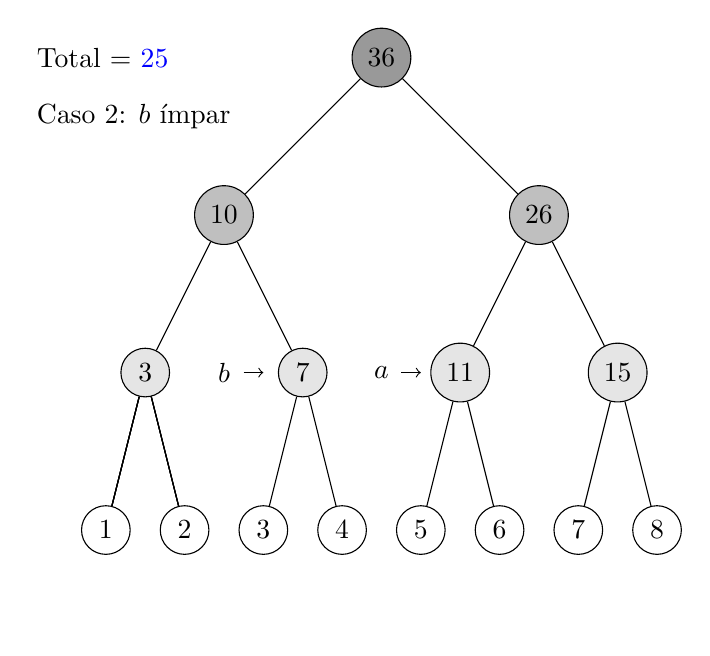
\begin{tikzpicture}
            \node[anchor=west] at (0, 6) { Total = \textcolor{blue}{$25$} };
            \node[anchor=west] at (0, 5.25) { Caso 2: $b$ ímpar };

            \node at (4.5, 2) { $a$ };
            \node at (2.5, 2) { $b$ };
            \node[opacity=0] at (3, -1) { $a$ };
            \node[opacity=0] at (6, -1) { $b$ };

            \draw[->] (4.75, 2) -- (5, 2);
            \draw[->] (2.75, 2) -- (3, 2);

            \node[draw,circle] (A1) at (1, 0) { 1 };
            \node[draw,circle] (A2) at (2, 0) { 2 };
            \node[draw,circle] (A3) at (3, 0) { 3 };
            \node[draw,circle] (A4) at (4, 0) { 4 };
            \node[draw,circle] (A5) at (5, 0) { 5 };
            \node[draw,circle] (A6) at (6, 0) { 6 };
            \node[draw,circle] (A7) at (7, 0) { 7 };
            \node[draw,circle] (A8) at (8, 0) { 8 };

            \node[draw,circle,fill=gray!20] (B1) at (1.5, 2) { 3 };
            \node[draw,circle,fill=gray!20] (B2) at (3.5, 2) { 7 };
            \node[draw,circle,fill=gray!20] (B3) at (5.5, 2) { 11 };
            \node[draw,circle,fill=gray!20] (B4) at (7.5, 2) { 15 };

            \node[draw,circle,fill=gray!50] (C1) at (2.5, 4) { 10 };
            \node[draw,circle,fill=gray!50] (C2) at (6.5, 4) { 26 };

            \node[draw,circle,fill=gray!80] (D1) at (4.5, 6) { 36 };

            \draw (A1) -- (B1);
            \draw (A2) -- (B1);
            \draw (A3) -- (B2);
            \draw (A4) -- (B2);
            \draw (A5) -- (B3);
            \draw (A6) -- (B3);
            \draw (A7) -- (B4);
            \draw (A8) -- (B4);
            \draw (A1) -- (B1);
            \draw (A2) -- (B1);
            \draw (A1) -- (B1);
            \draw (A2) -- (B1);
            \draw (A1) -- (B1);
            \draw (A2) -- (B1);
            \draw (B1) -- (C1);
            \draw (B2) -- (C1);
            \draw (B3) -- (C2);
            \draw (B4) -- (C2);
            \draw (C1) -- (D1);
            \draw (C2) -- (D1);
        \end{tikzpicture}
    \end{figure}

\end{frame}

\begin{frame}[fragile]{Visualização de RSQ(2, 6)}

    \begin{figure}
        \centering

        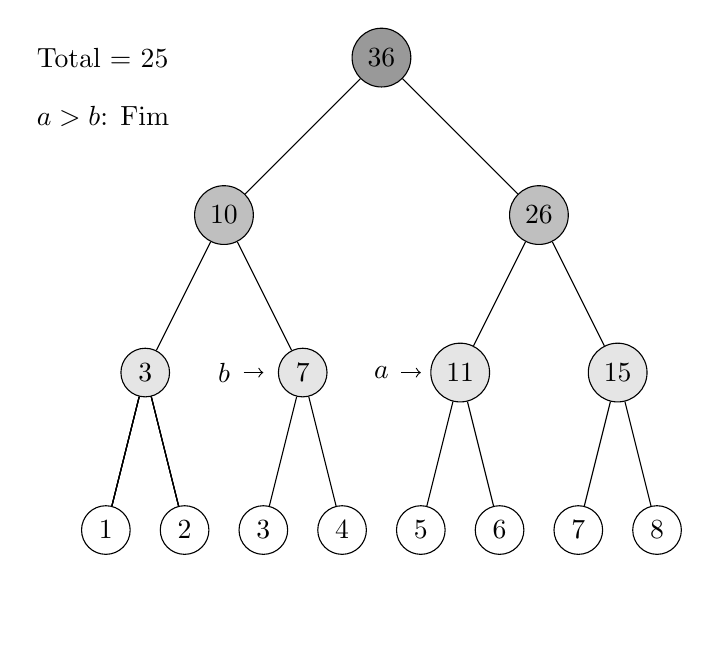
\begin{tikzpicture}
            \node[anchor=west] at (0, 6) { Total = \textcolor{black}{$25$} };
            \node[anchor=west] at (0, 5.25) { $a > b$: Fim };

            \node at (4.5, 2) { $a$ };
            \node at (2.5, 2) { $b$ };
            \node[opacity=0] at (3, -1) { $a$ };
            \node[opacity=0] at (6, -1) { $b$ };

            \draw[->] (4.75, 2) -- (5, 2);
            \draw[->] (2.75, 2) -- (3, 2);

            \node[draw,circle] (A1) at (1, 0) { 1 };
            \node[draw,circle] (A2) at (2, 0) { 2 };
            \node[draw,circle] (A3) at (3, 0) { 3 };
            \node[draw,circle] (A4) at (4, 0) { 4 };
            \node[draw,circle] (A5) at (5, 0) { 5 };
            \node[draw,circle] (A6) at (6, 0) { 6 };
            \node[draw,circle] (A7) at (7, 0) { 7 };
            \node[draw,circle] (A8) at (8, 0) { 8 };

            \node[draw,circle,fill=gray!20] (B1) at (1.5, 2) { 3 };
            \node[draw,circle,fill=gray!20] (B2) at (3.5, 2) { 7 };
            \node[draw,circle,fill=gray!20] (B3) at (5.5, 2) { 11 };
            \node[draw,circle,fill=gray!20] (B4) at (7.5, 2) { 15 };

            \node[draw,circle,fill=gray!50] (C1) at (2.5, 4) { 10 };
            \node[draw,circle,fill=gray!50] (C2) at (6.5, 4) { 26 };

            \node[draw,circle,fill=gray!80] (D1) at (4.5, 6) { 36 };

            \draw (A1) -- (B1);
            \draw (A2) -- (B1);
            \draw (A3) -- (B2);
            \draw (A4) -- (B2);
            \draw (A5) -- (B3);
            \draw (A6) -- (B3);
            \draw (A7) -- (B4);
            \draw (A8) -- (B4);
            \draw (A1) -- (B1);
            \draw (A2) -- (B1);
            \draw (A1) -- (B1);
            \draw (A2) -- (B1);
            \draw (A1) -- (B1);
            \draw (A2) -- (B1);
            \draw (B1) -- (C1);
            \draw (B2) -- (C1);
            \draw (B3) -- (C2);
            \draw (B4) -- (C2);
            \draw (C1) -- (D1);
            \draw (C2) -- (D1);
        \end{tikzpicture}
    \end{figure}

\end{frame}
